% Original study schematic; no claim of a new architecture or causal feedback.
\documentclass[tikz,border=2pt]{standalone}
\usepackage{fontspec}
\setsansfont{Arial}
\usetikzlibrary{arrows.meta,shapes.misc}
\definecolor{blue}{HTML}{0072B2}
\definecolor{orange}{HTML}{B36B00}
\definecolor{ink}{HTML}{303843}
\begin{document}
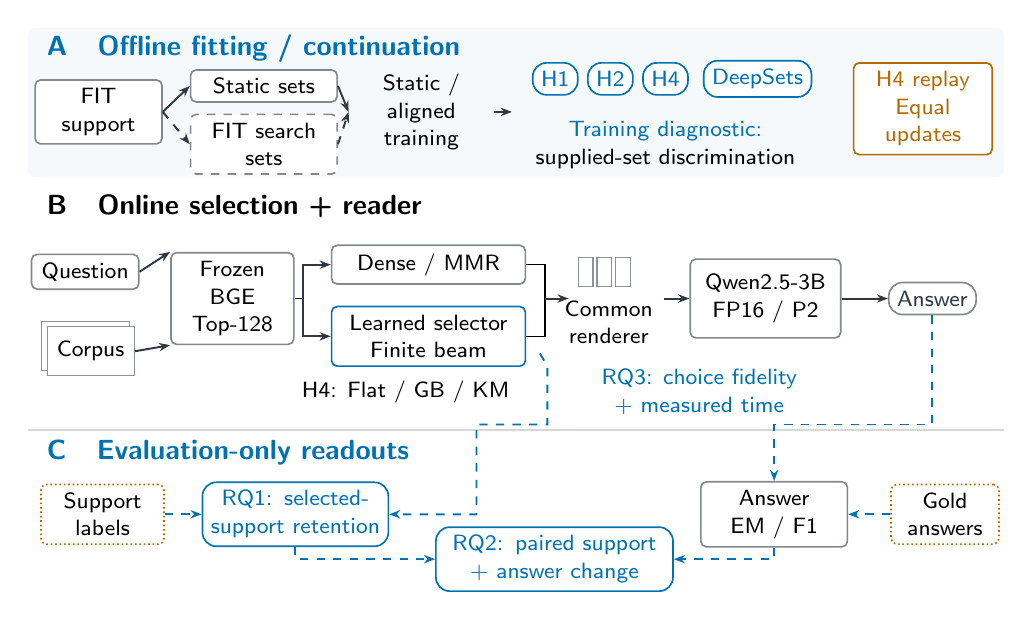
\begin{tikzpicture}[x=1cm,y=1cm,font=\sffamily\fontsize{8.5}{10}\selectfont,
 box/.style={draw=ink!60,fill=white,rounded corners=2pt,align=center,inner sep=3pt,line width=.6pt},
 badge/.style={box,rounded corners=5pt,draw=blue,text=blue,inner sep=3pt},
 flow/.style={-{Stealth[length=4pt]},line width=.7pt,draw=ink},
 readout/.style={flow,draw=blue,dashed},
 head/.style={anchor=west,font=\sffamily\bfseries\fontsize{10}{11}\selectfont}]
\path[use as bounding box] (0,0) rectangle (12.4,7.3);
\fill[blue!4,rounded corners=3pt] (0,5.4) rectangle (12.4,7.3);
\node[head,text=blue] at (.12,7.04) {A\quad Offline fitting / continuation};
\node[box,text width=1.4cm] (sup) at (.9,6.23) {FIT support};
\node[box,text width=1.65cm] (static) at (3.0,6.56) {Static sets};
\node[box,dashed,text width=1.65cm] (search) at (3.0,5.82) {FIT search sets};
\draw[flow] (sup.east)--(static.west);
\draw[flow,dashed] (sup.east)--(search.west);
\node[align=center,text width=1.6cm] (training) at (5.0,6.23) {Static / aligned\\training};
\draw[flow] (static.east)--(training.west);
\draw[flow,dashed] (search.east)--(training.west);
\foreach \x/\label in {6.7/H1,7.4/H2,8.1/H4,9.27/DeepSets}
 \node[badge] at (\x,6.65) {\label};
\draw[flow] (training.east)--(6.15,6.23);
\node[align=center,text width=4.1cm] at (8.1,5.81) {\textcolor{blue}{Training diagnostic:}\\supplied-set discrimination};
\node[box,draw=orange,text=orange,text width=1.55cm] at (11.37,6.27) {H4 replay\\Equal updates};

\node[head] at (.12,5.03) {B\quad Online selection + reader};
% Query and corpus: a query card over original stacked document sheets.
\node[box,text width=1.15cm] (query) at (.73,4.2) {Question};
\draw[ink!55,fill=white] (.18,2.95) rectangle (1.29,3.57);
\draw[ink!55,fill=white] (.25,2.88) rectangle (1.36,3.5);
\node[align=center] at (.8,3.19) {Corpus};
\node[box,text width=1.35cm,minimum height=1.03cm] (bge) at (2.6,3.86) {Frozen BGE\\Top-128};
\draw[flow] (query.east)--(bge.north west);
\draw[flow] (1.36,3.19)--(bge.south west);
\node[box,text width=2.25cm] (base) at (5.09,4.29) {Dense / MMR};
\node[box,draw=blue,text width=2.25cm] (learn) at (5.09,3.38) {Learned selector\\Finite beam};
\coordinate (split) at (3.5,3.86);
\draw (bge.east)--(split);
\draw[flow] (split)|-(base.west);
\draw[flow] (split)|-(learn.west);
\node[align=center] at (4.8,2.67) {H4: Flat / GB / KM};
\coordinate (merge) at (6.57,3.86);
\draw (base.east)-|(merge); \draw (learn.east)-|(merge);
% Small adjacent evidence cards suggest a set; only the common renderer is named.
\foreach \x in {6.99,7.23,7.47} \draw[ink!55,fill=white] (\x,4.01) rectangle +(0.19,.37);
\node[align=center,text width=1.5cm] (render) at (7.38,3.56) {Common\\renderer};
\draw[flow] (merge)--(6.87,3.86);
\node[box,text width=1.7cm,minimum height=1.0cm] (reader) at (9.37,3.86) {Qwen2.5-3B\\FP16 / P2};
\draw[flow] (8.08,3.86)--(reader.west);
\node[badge,text=ink,draw=ink!60] (answer) at (11.49,3.86) {Answer};
\draw[flow] (reader)--(answer);
\node[text=blue,align=center] at (8.53,2.67) {RQ3: choice fidelity\\+ measured time};

\draw[ink!20] (0,2.19)--(12.4,2.19);
\node[head,text=blue] at (.12,1.9) {C\quad Evaluation-only readouts};
\node[box,draw=orange,densely dotted,text width=1.35cm] (lab) at (.95,1.12) {Support labels};
\node[badge,text width=2.15cm] (rq1) at (3.4,1.12) {RQ1: selected-\\support retention};
\node[badge,text width=2.8cm] (rq2) at (6.69,.55) {RQ2: paired support\\+ answer change};
\node[box,text width=1.65cm] (em) at (9.48,1.12) {Answer EM / F1};
\node[box,draw=orange,densely dotted,text width=1.16cm] (gold) at (11.65,1.12) {Gold answers};
\draw[readout] (lab)--(rq1);
\draw[readout] (gold)--(em);
\draw[readout] (rq1.south)|-(rq2.west);
\draw[readout] (em.south)|-(rq2.east);
\draw[readout] (render.south west)--(6.6,3.0)--(6.6,2.26)--(5.7,2.26)--(5.7,1.12)--(rq1.east);
\draw[readout] (answer.south)--(11.49,2.26)--(9.48,2.26)--(em.north);
\end{tikzpicture}
\end{document}
